\chapter{Supplementary Material for Contribution 4 (RQ4)}\label{app:rq4}

The content of this appendix is based on \citet{GOLAB2025134385}. It supplements the results presented in Section~\ref{sec:rq4_results}.

This appendix presents results from the integration of the spatio-temporal commercial \ac{BEV} fleet charging demand profiles---developed as part of this dissertation---into an electricity market model for dispatch and redispatch optimization. In the European electricity market framework, \textit{dispatch} refers to the scheduling of generation and flexible loads in the day-ahead market clearing, which is performed at the bidding zone level without considering internal transmission constraints. \textit{Redispatch} is the subsequent corrective adjustment of generation and load schedules to resolve congestion within the transmission grid, accounting for the physical network topology. The dispatch and redispatch models were developed and implemented by Christoph Loschan; the results shown here illustrate how the bottom-up charging demand profiles interact with market clearing and congestion management mechanisms. Three electrification scenarios are considered for 2040: \textit{LOW} (30\% \ac{HDT} electrification), \textit{MEDIUM} (50\%), and \textit{HIGH} (100\%), with light-duty vehicles and buses at 100\% electrification in all scenarios (see Table~\ref{tab:parameters_scenario}). For each scenario, three case studies are compared: \textit{Baseline} (inflexible charging at constant power), \textit{Dispatch} (charging flexibility coordinated in the day-ahead market to minimize dispatch costs), and \textit{Redispatch} (charging flexibility used for congestion management in the transmission grid).

\section{Impact of Market Participation on Dispatch}\label{app:rq4_dispatch}

When the commercial \ac{BEV} fleet's charging flexibility is utilized in the day-ahead market clearing, charging demand shifts toward hours of low electricity prices. During workdays, two price lows occur around noon and around midnight; these coincide with increased charging peaks. The nighttime peak during workdays increases by 80\% compared to the \textit{Baseline} charging profile. During weekends, significant price lows around noon create peak load values roughly eight times greater than the \textit{Baseline} charging demand at that hour.

Figure~\ref{fig:app_rq4_annual_duration} shows the annual duration curve of total electricity demand in Austria for 2040 under the different case studies and electrification scenarios. The price-oriented dispatch coordination increases peak load values by up to 24\% compared to the \textit{Baseline} and decreases the load during hours of higher prices. This effect intensifies with rising electrification rates.

\begin{figure}[H]
    \centering
    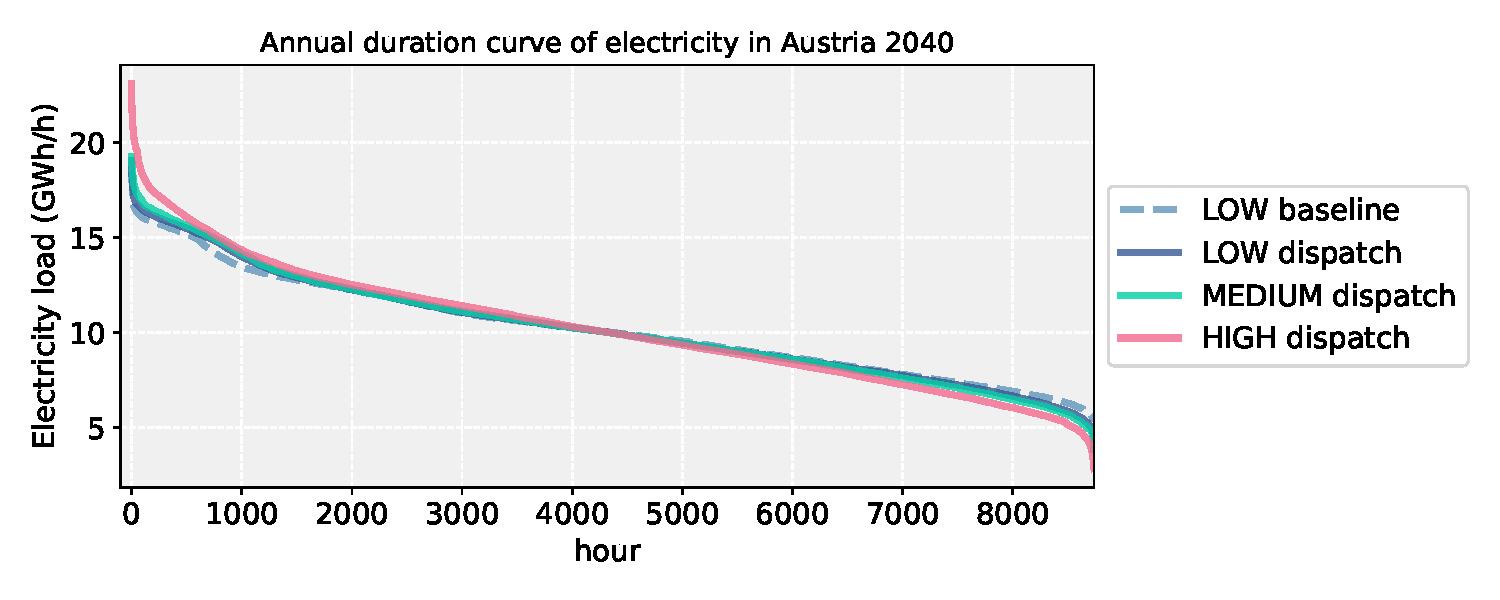
\includegraphics[width=0.9\textwidth]{graphics/paper_4/annual_duration_curve.pdf}
    \caption{Annual duration curve of electricity demand in Austria in 2040 for different case studies and electrification scenarios.}
    \label{fig:app_rq4_annual_duration}
\end{figure}

\section{Participation in Redispatch Measures}\label{app:rq4_redispatch}

Figure~\ref{fig:app_rq4_redispatch_profile} displays the aggregate weekly charging demand profile resulting from the participation of the commercial \ac{BEV} fleet in congestion management. The resulting load peaks are significantly lower than in the \textit{Dispatch} case study and, on average, do not significantly exceed the levels of the \textit{Baseline} load profile. On weekend days, the charging load is shifted to around noon, increasing the \textit{Baseline} load by 68\%---substantially less than the roughly eightfold increase observed in the \textit{Dispatch} case.

In contrast to the dispatch optimization, where charging processes are aggregated to the bidding zone level, the geographic variations are particularly relevant to the redispatch modeling, where the topology of the transmission grid and geographically varying dispatch and load centers are important factors.

\begin{figure}[H]
    \centering
    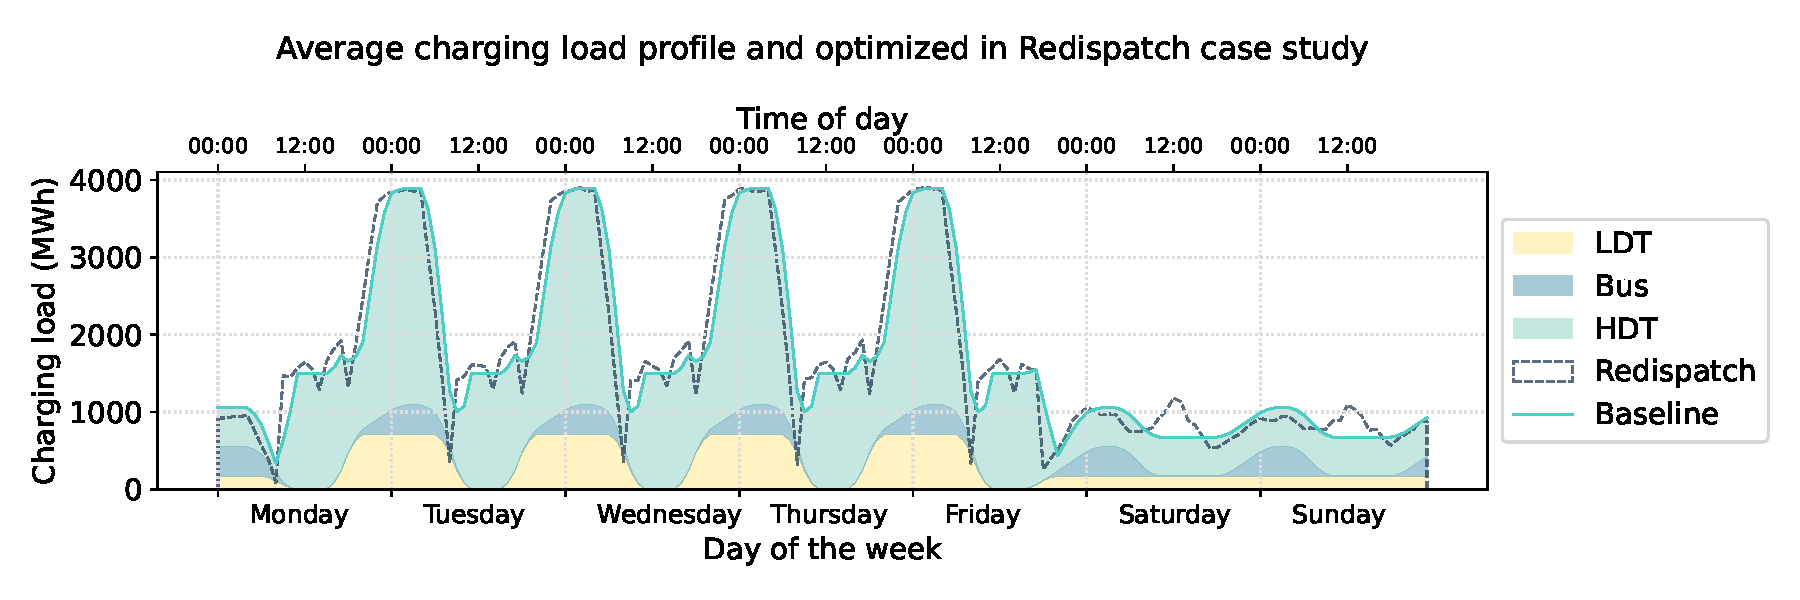
\includegraphics[width=\textwidth]{graphics/paper_4/average_load_profile_redispatch.pdf}
    \caption{Aggregated charging demand profile of the commercial \ac{BEV} fleet in the \textit{Baseline} and \textit{Redispatch} case studies.}
    \label{fig:app_rq4_redispatch_profile}
\end{figure}

\section{Spatial Variation in Redispatch Charging Profiles}\label{app:rq4_spatial}

Figure~\ref{fig:app_rq4_shifted_profiles} displays the average weekly charging profiles at all nodes representing the Austrian transmission grid. Compared to the aggregate load profile in Figure~\ref{fig:app_rq4_redispatch_profile}, significant variations are visible in both the absolute magnitude of the load profiles and in the shape of the curves, reflecting location-specific grid constraints and generation patterns.

\begin{figure}[H]
    \centering
    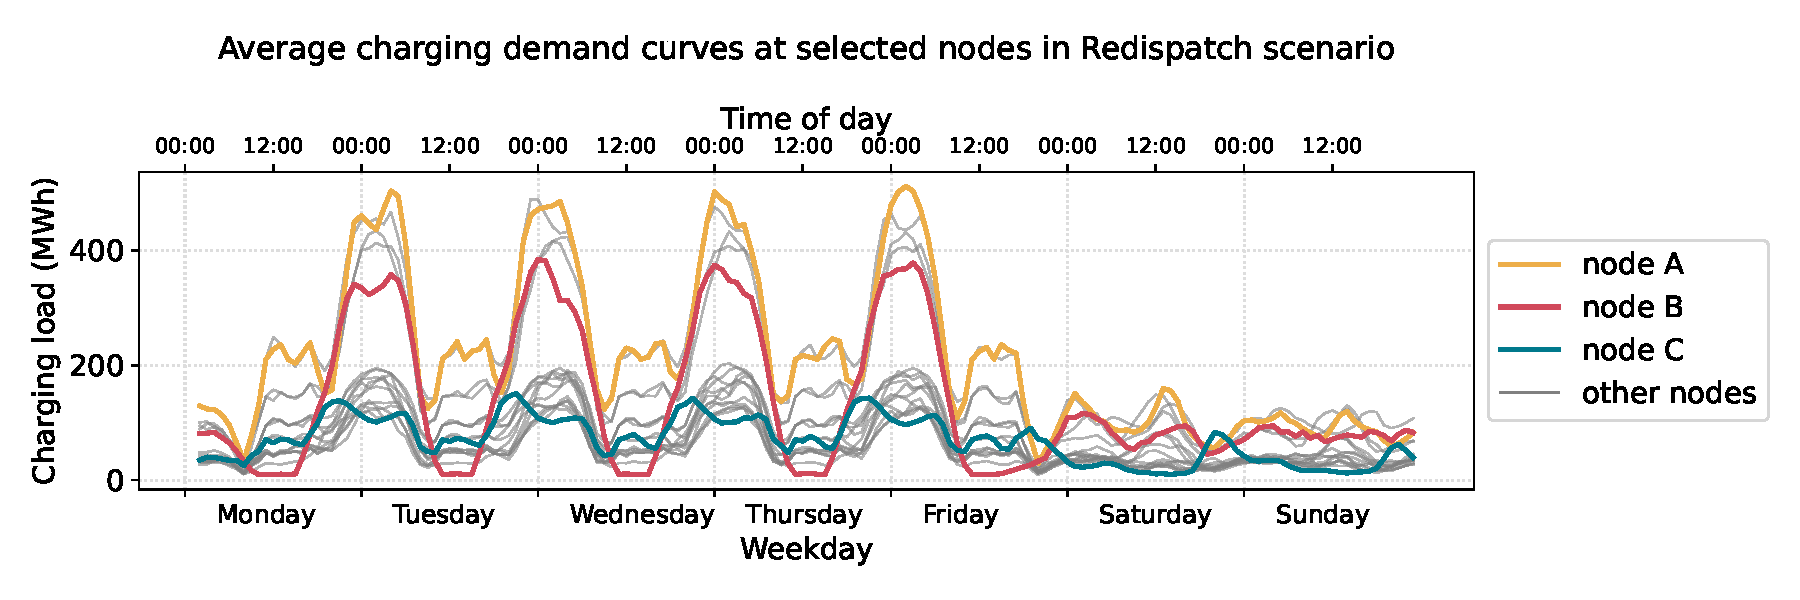
\includegraphics[width=\textwidth]{graphics/paper_4/shifted_load_profiles.pdf}
    \caption{Charging load curves resulting from participation of the commercial \ac{BEV} fleet in redispatch at different nodes in the Austrian transmission grid.}
    \label{fig:app_rq4_shifted_profiles}
\end{figure}

Three nodes are selected to illustrate the geographic differences in detail (Figure~\ref{fig:app_rq4_node_map}):

\begin{figure}[H]
    \centering
    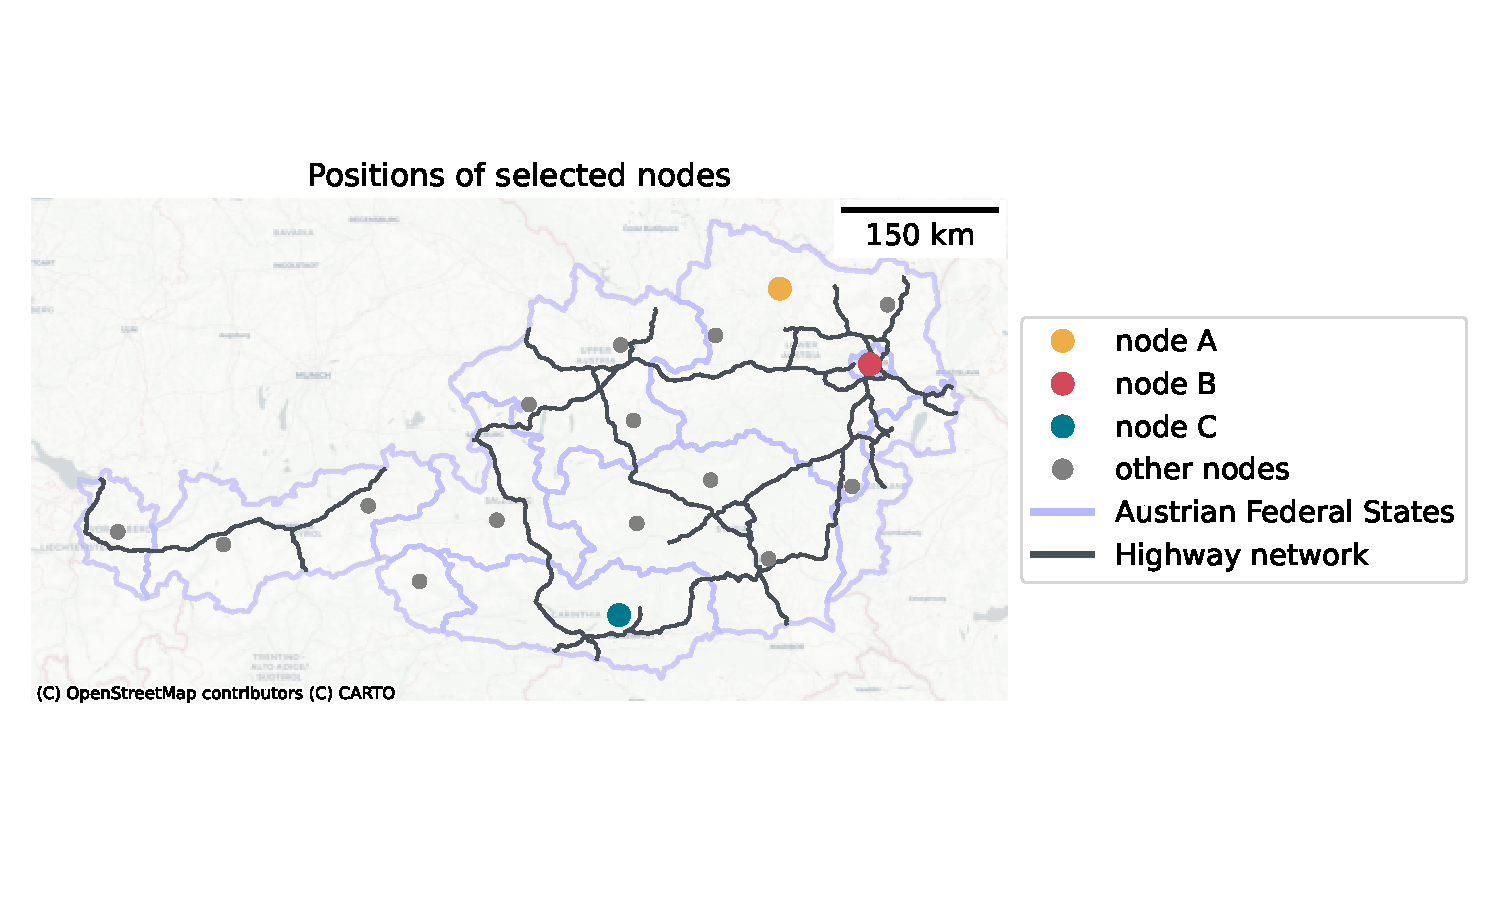
\includegraphics[width=0.9\textwidth]{graphics/paper_4/selected_nodes.pdf}
    \caption{Geographical allocation of selected nodes representing the Austrian transmission grid in the redispatch model.}
    \label{fig:app_rq4_node_map}
\end{figure}

The corresponding charging profiles are shown in Figure~\ref{fig:app_rq4_selected_nodes}.

\textbf{Node~A (Lower Austria):} Lower Austria is the federal state with the second-highest population and the largest area, as well as the highest total kilometers of highway and motorway network. Relatively high daytime peak loads are visible. When the commercial \ac{BEV} fleet participates in redispatch, the charging profile does not significantly deviate from the \textit{Baseline}; however, the absolute peaks during noon (highway charging) and at night around midnight increase. On Saturdays, peaks emerge similarly to the aggregate profile.

\textbf{Node~B (Vienna):} Vienna has the highest population and population density, consisting almost exclusively of urban area. This is reflected in the high share of light-duty truck charging demand and the lowest daytime demand for charging at highway service areas. Similarly to Node~A, no significant deviations from the \textit{Baseline} profile are observed under redispatch.

\textbf{Node~C (Southern Austria, near Italy):} The shape of the charging profile is significantly altered when the commercial \ac{BEV} fleet participates in redispatch measures. During workdays, the nighttime charging load shifts substantially to earlier times. During weekends, load peaks appear around 6~pm---a pattern distinct from other regions---reflecting the influence of local grid topology and cross-border power flows.

\begin{figure}[H]
    \centering
    \begin{minipage}[t]{\textwidth}
        \centering
        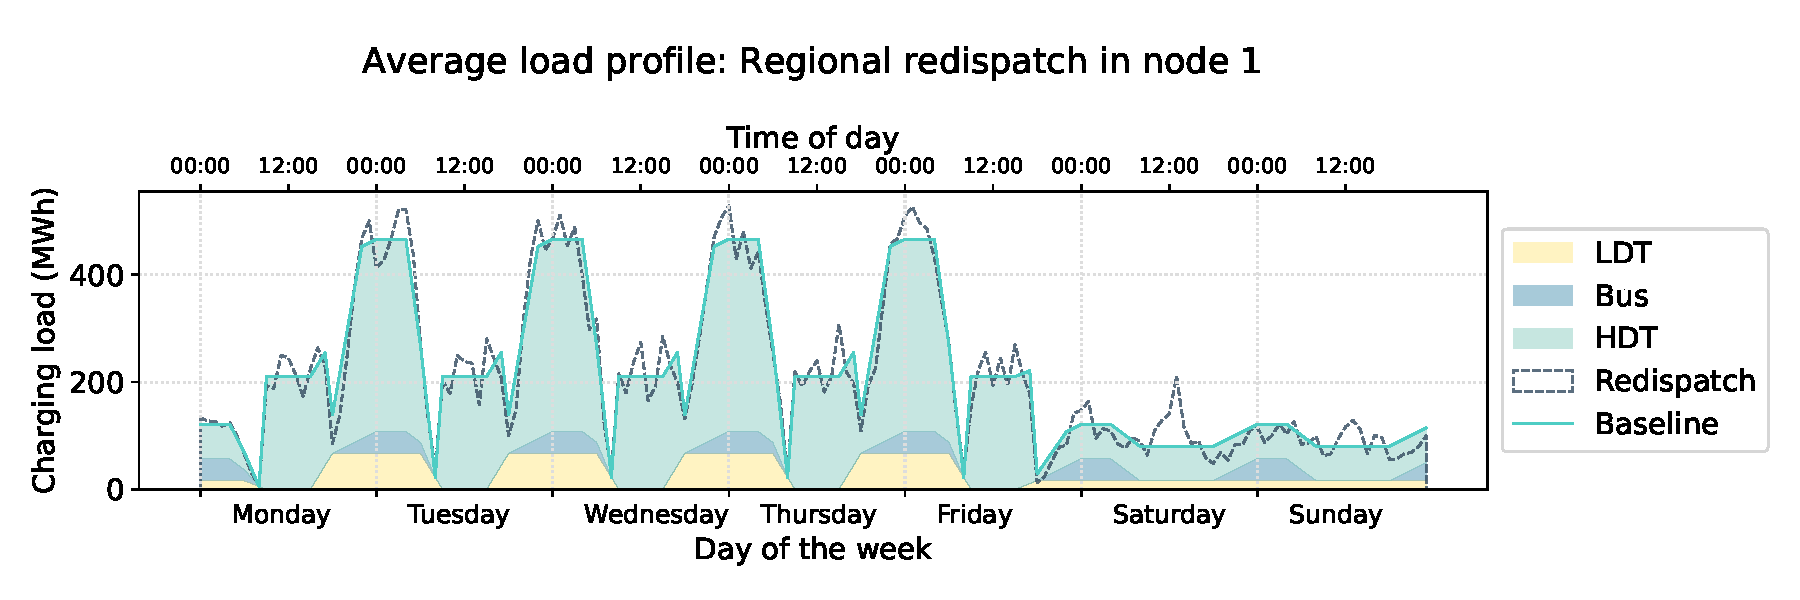
\includegraphics[width=\linewidth]{graphics/paper_4/NOEaverage_load_profile.pdf}
    \end{minipage}
    \begin{minipage}[t]{\textwidth}
        \centering
        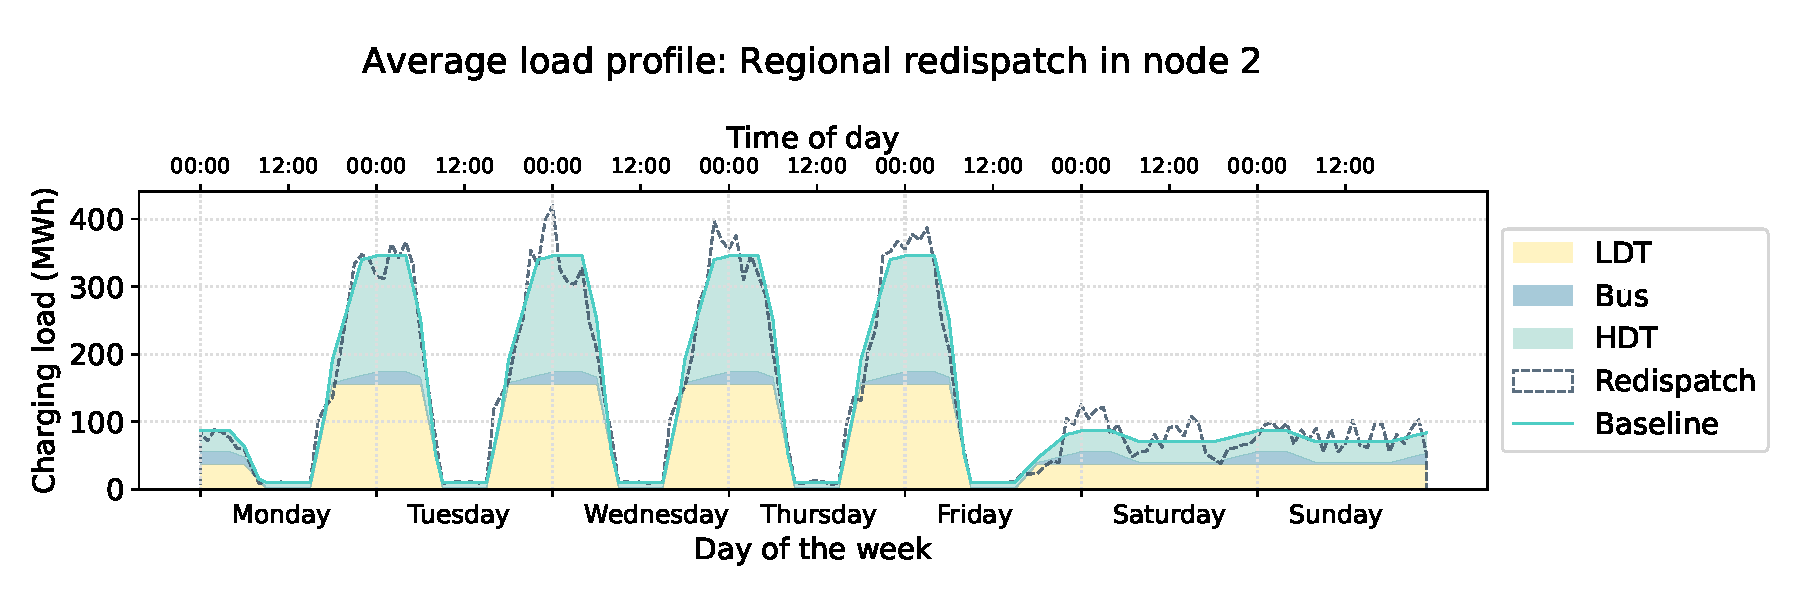
\includegraphics[width=\linewidth]{graphics/paper_4/Waverage_load_profile.pdf}
    \end{minipage}
    \begin{minipage}[t]{\textwidth}
        \centering
        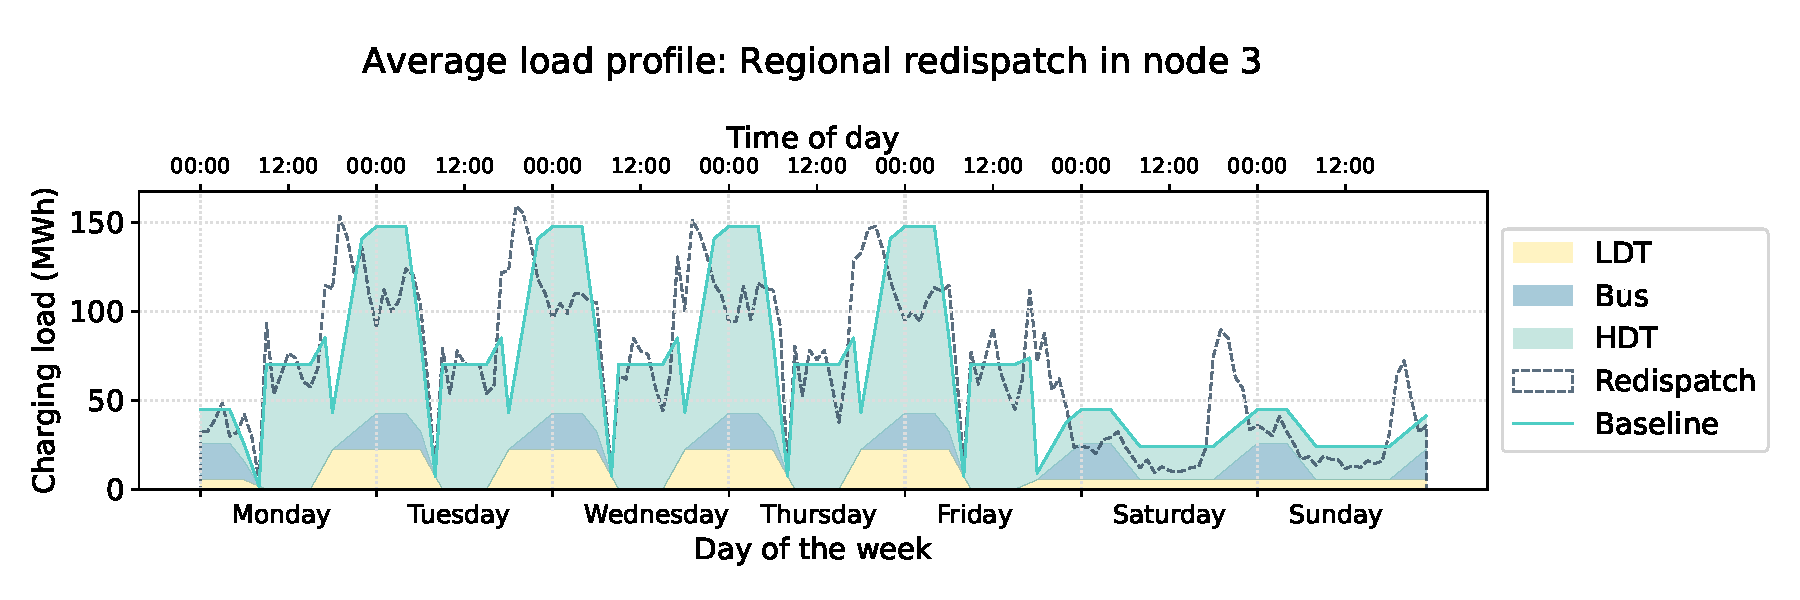
\includegraphics[width=\linewidth]{graphics/paper_4/KTN_waverage_load_profile.pdf}
    \end{minipage}
    \caption{Average weekly charging profiles at three selected nodes for the \textit{Baseline} and \textit{Redispatch} case studies: Node~A (Lower Austria, top), Node~B (Vienna, middle), and Node~C (Southern Austria, bottom).}
    \label{fig:app_rq4_selected_nodes}
\end{figure}

\section{Comparison of Redispatch Costs}\label{app:rq4_costs}

Figure~\ref{fig:app_rq4_costs} compares the redispatch costs across the three case studies and electrification scenarios. Three key observations emerge:

First, in the \textit{Baseline} case, the increasing electrification of the commercial fleet has a limited impact on redispatch costs. The costs decrease slightly by 4~million~euros between the \textit{LOW} and \textit{HIGH} scenarios.

Second, the increasing electrification of the truck fleet substantially affects the redispatch costs when charging flexibility is utilized in the dispatch. At an electrification rate of 30\% of the \ac{HDT} fleet, costs increase by approximately 40\% between the initial (\textit{Baseline}) charging strategy and dispatch-coordinated charging. This demonstrates that market-price-based flexibility utilization, which ignores transmission grid topology, increases grid congestion and the associated redispatch costs.

Third, the coordination of charging profiles to minimize redispatch costs effectively decreases the costs by approximately 30--35\% relative to the \textit{Baseline} case, highlighting the value of grid-aware charging coordination.

\begin{figure}[H]
    \centering
    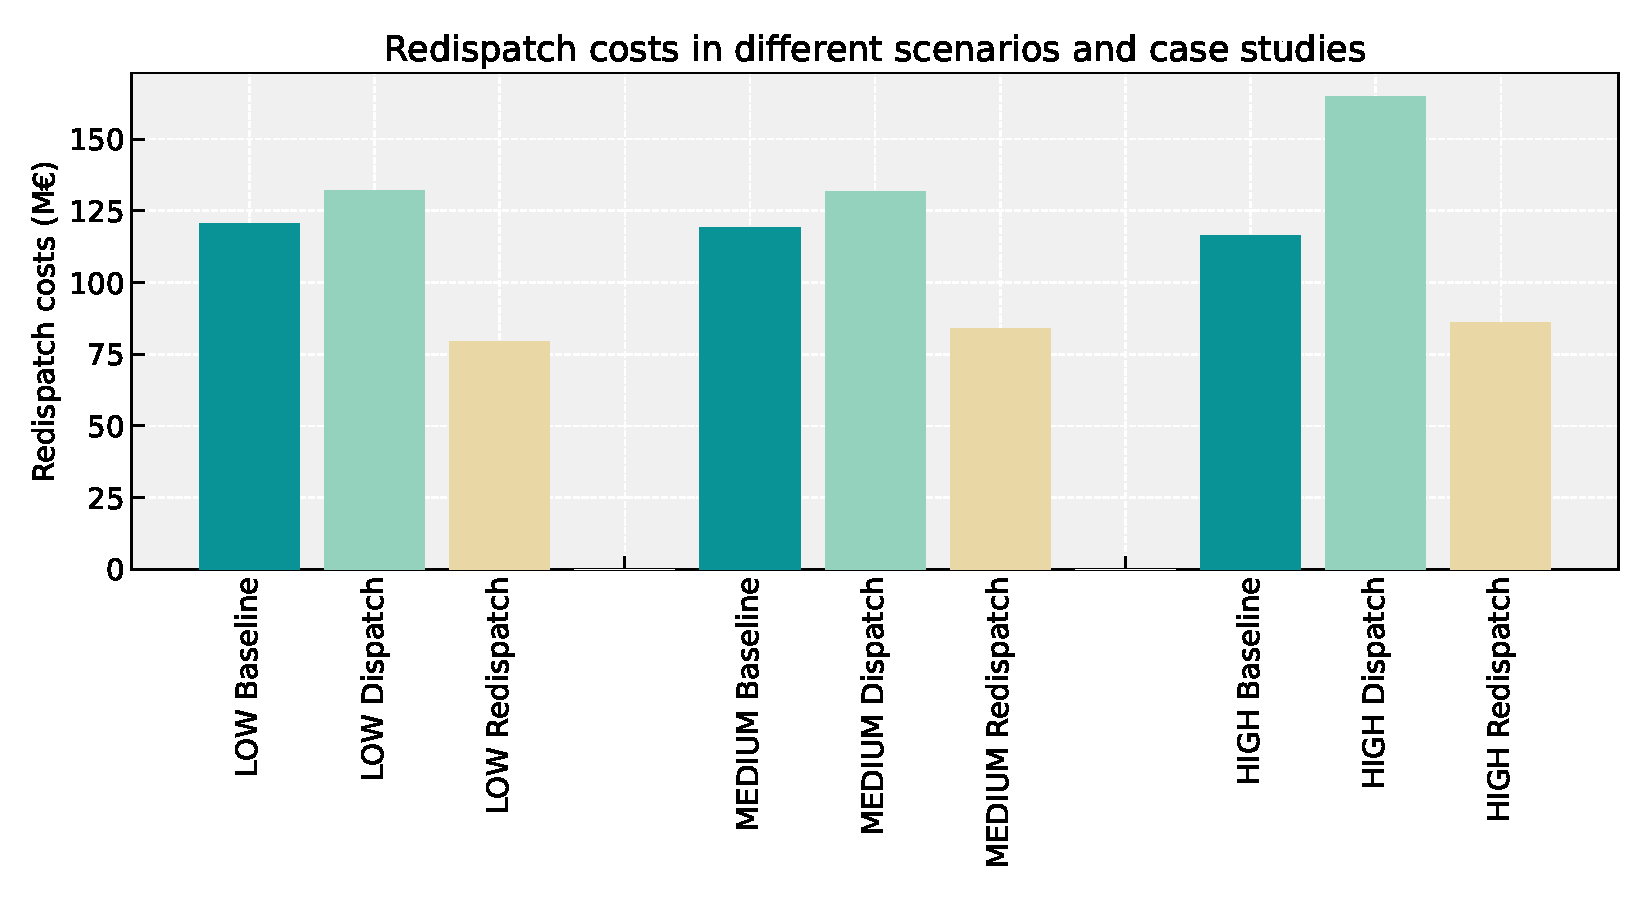
\includegraphics[width=0.8\textwidth]{graphics/paper_4/costs.pdf}
    \caption{Comparison of redispatch costs for different electrification scenarios and case studies for Austria in 2040.}
    \label{fig:app_rq4_costs}
\end{figure}

These results emphasize that with the increasing electrification of the transport sector, the cross-sectoral consideration of electricity and transport becomes increasingly important. The activation of demand-side flexibility of the charging processes is not weighted by any additional cost parameter in the dispatch objective and is exclusively limited by plug-in times and charging capacities. This implies that if fleet operators coordinate fleet charging based on market prices alone, substantial peak loads occur and redispatch costs increase. Targeted regulatory incentives---such as peak or dynamic pricing---are needed, and these would have to be dependent on the geographical allocation to be effective.
